\chapter{Método de Kapitza en la dinámica semiclásica del electrón en la red de enlace fuerte sometido a potenciales rápidamente oscilantes}\label{cap:9} 

En este capítulo se estudia la dinámica semiclásica de un electrón en la red en presencia de un campo externo rápidamente oscilante, los resultados que se obtienen en este capítulo forman parte de los resultados de este proyecto de grado. Para el desarrollo de estos cálculos se hace uso del método semiclásico para modelar la dinámica de un electrón en una red de \textit{Tight Binding} en presencia de un campo externo, combinado con el método de Kapitza para la dinámica clásica de una partícula en presencia de fuerzas rápidamente oscilantes. Se sigue el procedimiento de Maricq para resolver la dinámica del electrón en una red de \textit{Tight Binding} y en presencia de un potencial externo rápidamente oscilante \cite{maricq}\cite{mart2014}.

%%%%%%%%%%%%%%%%%%%%%%%%%%%%%%%%%%%%%%%%%%

Se presenta el problema de un electrón en una red unidimensional, bajo la influencia de un campo eléctrico externo inhomogéneo y rápidamente oscilante. Esto es, la frecuencia de oscilación de este campo externo es mucho mayor que $\omega_{0}$. Las perturbaciones dependientes del tiempo, como la que se presenta, han sido estudiadas extensamente \cite{Dunlap}\cite{mart2014}. Si el movimiento está gobernado por las leyes de la mecánica clásica y la perturbación es rápida, intensa y periódica, existe un método desarrollado por Kapitza \cite{kapitza} y que se puede encontrar en el libro de Mecánica de Landau \cite{landau} que muestra es posible separar el movimiento en dos escalas de tiempo: una lenta gobernada por el sistema y una rápida como consecuencia de la perturbación. El uso de este modelo permite encontrar una dinámica efectiva independiente del tiempo para la partícula.

La dinámica de un electrón en la red, en presencia de un campo externo, puede ser estudiada a través de modelos semiclásicos \cite{ashc}, tal como se ha tratado en la sección \ref{cap:7} combinado con el metodo de Kapitza tratado en la sección \ref{cap:6}. En esta sección, se incluirán los resultados del modelo de \textit{Tight Binding} para hallar un modelo semiclásico que describa la dinámica de electrón.

Sea $U(x)$ un potencial que no depende del tiempo y $V(x,t)$ un potencial inhomogéneo que varía rápidamente en el tiempo ($\omega \gg \omega_o$). Las ecuaciones de movimiento del electrón en el modelo semiclásico están dadas por las siguientes ecuaciones:

\begin{equation}\label{eq:9.1}
    \dot{k}=\frac{-dU(x)}{dx}+f(x,t)
\end{equation}

\begin{equation}\label{eq:9.2}
    \dot{x}=2Aa\sin(ak)
\end{equation}
    
Donde la fuerza se ha definido como $f(x,t)=-\partial_x V(x,t)$. Se escribe la fuerza externa como una serie de Fourier (ecuación \ref{eq:9.3}) y se imponen las siguientes condiciones sobre ella:

\begin{enumerate}
    \item El promedio de $f(x,t)$ en un periodo de oscilación rápida es $\overline{f(x,t)}=0$
   \item $f_n(x)=f_{-n}(x)$ (Paridad)
\end{enumerate}

\begin{equation} \label{eq:9.3}
    f(x,t)=\sum_{-\infty}^{\infty} f_n(x) e^{i n\omega t}
\end{equation}
    
Se puede representar el movimiento total de la partícula como la suma de dos movimientos independientes: uno rápido ($\xi(t)$), de amplitud pequeña, y otro lento ($X(t)$) de mayor amplitud \cite{landau}. Esta situación se describe de la siguiente manera:
   
\begin{equation}\label{eq:9.4}
    x=X(t)+\xi(t)
\end{equation}
   
\begin{equation}\label{eq:9.5}           
    k=K(t)+\eta(t)
\end{equation}
    
Donde $\overline{\eta}=\overline{\xi}=0$. Se derivan las ecuaciones \ref{eq:9.4} y \ref{eq:9.5} para obtener las velocidades del sistema. Y, al derivar de nuevo para obtener la aceleración, se acoplan ambas ecuaciones para obtener la aceleración del electrón:
    
\begin{equation}\label{eq:9.6}
    \dot{X}+\dot{\xi}=2Aa\sin(ak)
\end{equation}
    
\begin{equation}\label{eq:9.7}               \dot{K}+\dot{\eta}=-\frac{dU}{dx}+f(x,t)
\end{equation}

\begin{equation}\label{eq:9.8}
    \ddot{X}+\ddot{\xi}=2Aa\cos(ak)\times\dot{k}
\end{equation}

\section{Separación de movimientos rápido y lento}\label{cap:9.1.1}

Se obtuvo una expresión para la aceleración, la cual no puede ser separada (de momento) en movimientos rápido y lento. Se sigue un procedimiento que permite separar estos movimientos de acuerdo al método usado por Kapitza \cite{kapitza}. En primer lugar, se sustituye las ecuaciones \ref{eq:9.1} y \ref{eq:9.5} en \ref{eq:9.8}:
 
\begin{equation}\label{eq:9.9}
    \ddot{X}+\ddot{\xi}=2Aa^2\cos((K+\eta)a)\times(-\frac{dU}{dx}+f(x,t))
\end{equation}
    
Usando la siguiente identidad trigonométrica y sustituyendo en la ecuación \ref{eq:9.9} se obtiene:

$$\cos(a+b)=\cos(a)\cos(b)-\sin(a)\sin(b)$$

\begin{equation}\label{eq:9.10}
    \ddot{X}+\ddot{\xi}=2Aa^2(\cos(Ka)\cos(\eta a)-\sin(Ka)\sin(\eta     a))\times(-\frac{dU}{dx}+f(x,t))
\end{equation}

 Siguiendo el procedimiento de Landau \cite{landau} se expande en serie de Taylor $\frac{dU}{dx}$ y $f(x,t)$ alrededor de $\xi=0$ a primer orden, para conocer como actúan estas fuerzas en la zona del movimiento oscilatorio rápido.

\begin{equation}\label{eq:9.11}
    \frac{dU}{dx}=\frac{dU}{dX}+\xi\frac{d^2U}{dX^2}
\end{equation}
    
\begin{equation}\label{eq:9.12}
    f(X,t)=f(X,t) + \xi \frac{\partial f(X,t)}{\partial X} 
\end{equation}

Sustituyendo la expresión \ref{eq:9.11} y \ref{eq:9.13} en \ref{eq:9.10} se obtiene lo siguiente: 
    
\begin{equation}\label{eq:9.13}
    \begin{split} 
        &\ddot{X}+\ddot{\xi}=2Aa^2\left(\cos(Ka)\cos(\eta a)-\sin(Ka)\sin(\eta a)\right)(-\frac{dU}{dX}-\xi\frac{d^2U}{dX^2}+ \\ &+f(X,t) + \xi \frac{\partial f(X,t)}{\partial X} )
    \end{split}
\end{equation}

Tomando $\xi$ muy pequeño, se pueden separar los movimientos rápido y lento como en las siguientes expresiones:

\begin{equation}\label{eq:9.14}
    \ddot{\xi}=2Aa^2\left(\cos(Ka)\cos(\eta a)-\sin(Ka)\sin(\eta a)\right)f(X,t)
\end{equation}

\begin{equation}\label{eq:9.15}
   \ddot{X}=2Aa^2\left(\cos(Ka)\cos(\eta a)-\sin(Ka)\sin(\eta a)\right)\left(-\frac{dU}{dX}-\xi\frac{d^2U}{dX^2} + \xi \frac{\partial f(X,t)}{\partial X} \right)
\end{equation}

Este producto se resuelve, para luego calcular el promedio para un periodo en la oscilación pequeña, donde se tiene que $\overline{\ddot{X}}=\ddot{X}$. Haciendo uso de los promedios calculados en el apéndice \ref{apendice:B.4}, se obtiene que la aceleración efectiva del electrón en la red, en presencia de un campo externo rápidamente oscilante, esta dado por:

\begin{equation}\label{eq:9.16}
 \ddot{X}= -2Aa^2\cos(Ka)\left[\left(1-\frac{a^2}{2}\sum_n \frac{f_n^2(X)}{\omega^2n^2}\right)\frac{dU}{dX}+2Aa^2\cos(Ka)\sum_n \frac{1}{2n^2\omega^2}\frac{\partial f_n^2(X)}{\partial X}\right]
\end{equation}

Donde $m^*=(2Aa^2\cos(Ka))^{-1}$ es la masa efectiva del electrón en la red de enlace fuerte, por lo tanto, la formula general para la aceleración efectiva es:

\begin{equation}\label{eq:9.17}
 \ddot{X}= -\frac{1}{m^*}\left(1-\frac{a^2}{2}\sum_n \frac{f_n^2(X)}{\omega^2n^2}\right)\frac{dU}{dX}-\frac{1}{2m^{*2}\omega^2}\sum_n \frac{1}{n^2}\frac{\partial f_n^2(X)}{\partial X}
\end{equation}

\section{Calculo del potencial efectivo}\label{cap:9.1.2}

De la ecuación \ref{eq:9.17} es posible obtener el potencial efectivo:

\begin{equation}\label{eq:9.18}
    U_{eff}= U(X)-\frac{a^2}{2\omega^2}\sum_n \frac{f_n^2(X)}{n^2}U(X)+\frac{1}{2m^{*}\omega^2}\sum_n \frac{f_n^2(X)}{n^2} 
\end{equation}

Estos resultados se asemejan a los obtenidos por Malay Bandyopadhyay et al. \cite{datta} salvo el segundo término, el cual se explica por la presencia de la relación de dispersión de \textit{Tight Binding} en las ecuaciones de movimiento del electrón. Obsérvese que debido al efecto de la fuerza oscilante, tendremos una corrección en el potencial experimentado por la partícula, cuyo valor, se ha aproximado hasta términos de $\omega^{-2}$.

Se observa que en el límite del continuo $m^* \rightarrow m$ y el potencial efectivo toma la forma exacta del resultado de Malay Bandyopadhyay et al.: 

\begin{equation}\label{eq:9.19}
    \lim_{a\rightarrow 0}U_{eff}= U(X)+\frac{1}{2m\omega^2}\sum_n \frac{f_n^2(X)}{n^2} 
\end{equation}

Este resultado difiere del obtenido por Martínez et al.(2014) \cite{mart2014}, se usó una aproximación diferente al del citado artículo para calcular el potencial efectivo, ya que se encontró que las variables $\eta$ y $\xi$ no son independientes entre sí, en consecuencia no se puede calcular los promedios por separado de los factores de la ecuación \ref{eq:9.15} para luego expandir el producto. 

\section{Obtención de una cantidad conservada en la dinámica del electrón en la red en presencia de un campo externo rápidamente oscilante}\label{cap:9.2}

Se ha hallado una expresión para la aceleración efectiva del electrón y el potencial efectivo del electrón. Se puede hallar además, tal como encontró Martínez et al. (2014) una cantidad conservada para el movimiento del electrón en este sistema.

Se comenzará calculando $\dot{X}/\dot{K}$ siguiendo procedimiento de Martínez (2014) \cite{mart2014}: 
\begin{equation}\label{eq:9.20}
    \frac{dX}{dK}=\frac{-2A\sin(Ka)\overline{\cos(\eta a)}}{-\frac{\partial U}{\partial X}+\xi \overline{\frac{\partial f(X)}{\partial X}}}
\end{equation}

Del apéndice \ref{apendice:B} se obtiene el siguiente resultado:

    \begin{equation}\label{eq:9.21}
        \overline{\xi \frac{\partial f(X,t)}{\partial X}}=2A\cos(Ka)\frac{\partial\overline{cos(\eta a)}}{\partial X}
    \end{equation}
 
 De la ecuación \ref{eq:9.20} se obtiene la forma del diferencial total $d\left(-2A\cos(Ka)\overline{\cos(\eta a)}+U(X)\right)$, tomando en cuenta el resultado \ref{eq:9.21} se encuentra que el diferencial total es idéntico a cero:
 
 \begin{equation}
    \begin{split}
     0&=\frac{\partial}{\partial X} \left(-2A\cos(Ka)\overline{cos(\eta a)}+U(X)\right)dX+\frac{\partial}{\partial K}\left(-2A\cos(Ka)\overline{cos(\eta a)}\right)\\
     &=d\left(2A\cos(Ka)\overline{cos(\eta a)}+U(X)\right)
     \end{split}
 \end{equation}
 
 Se encuentra una cantidad conservada para el electrón en el sistema que se denotará por $\mathcal{E}$
 
    
\begin{equation}\label{eq:9.24}
    \mathcal{E}=-2A\cos(aK)+U(X)+2Aa^2\cos(Ka)\sum_n\frac{f_n^2(X)}{2n^2\omega^2}
\end{equation}  

Cuyo resultado, coincide con el resultado del trabajo de Malay Bandyopadhyay et al. \cite{datta} para el Hamiltoniano efectivo, usando el método de \textit{Rahav et al.}. Se puede inferir que la cantidad que se conserva es en realidad el Hamiltoniano efectivo del electrón. El resultado \ref{eq:9.24} puede resumirse como: 

\begin{equation}\label{eq:9.25}
    H(X,K)=H_0(X,K)+\frac{1}{2\omega^2m^*}\sum_n\frac{f_n^2(X)}{n^2}
\end{equation}

Donde $H_0(X,K)$ es el Hamiltoniano en la red de \textit{Tight Binding} en ausencia del campo externo rápidamente oscilante.

\begin{equation}\label{eq:9.26}
    H_0(X,K)=-2A\cos(aK)+U(X)
\end{equation}


\section{Masa efectiva}

Es posible calcular la masa efectiva del electrón en este sistema ($m^{**}$) haciendo uso de la definición de masa efectiva.

\begin{equation}
    m^{**}=\frac{1}{2Aa^2\cos(Ka)}\left(1+\frac{a^2}{2}\sum_n \frac{f_n^2(X)}{\omega^2n^2}\right)
\end{equation}

Se obtiene además que en el limite del continuo la masa efectiva resulta ser la masa del electrón libre, como es de esperar.

\begin{equation}
    \lim_{a \rightarrow 0}m^{**}=m
\end{equation}

%%%%%%%%%%%%%%%%%%%%%%%%%%%%%%%%
\section{Aplicación del resultado semiclásico al caso lineal}

Se hace uso de los resultados generales obtenidos para modelar la dinámica del electrón en la red en presencia de un potencial eléctrico lineal que varia periódicamente con frecuencia $\omega$. El Hamiltoniano del electrón en este sistema es;

\begin{equation}\label{eq:9.28}
  H=-2A\cos(k a)+\epsilon x\cos{( \omega t)}  
\end{equation}


\begin{equation}\label{eq:9.29}
    f(x,t)=-\epsilon \cos(\omega t)
\end{equation}

Se observa que se trata de una fuerza que cumple con las condiciones en \ref{eq:9.3} %VERIFICAR%. 
Usando estas definiciones para $f(x,t)$ se obtiene que:

\begin{equation}\label{eq:9.30}
    f_{1}(x)=-\frac{\epsilon}{2}
\end{equation}

\begin{equation}\label{eq:9.31}
    U(x)=0
\end{equation}

    

El potencial efectivo está dado por la ecuación \ref{eq:9.32}. El potencial efectivo resulta ser constante, en consecuencia la fuerza efectiva es nula y su velocidad inicial permanece constante. Este resultado indica que el electrón se deslocaliza para periodos de movimiento lento, no efectúa oscilaciones alrededor de ningún punto de equilibrio estable y su posición no está acotada. 


\begin{equation}\label{eq:9.32}
    U_{eff} \approx \frac{1}{2m^*\omega^2} 2f_{1}^2(X)=\frac{\epsilon^2}{4m^*\omega^2}
\end{equation}


\section{Aplicación del resultado semiclásico al caso no lineal}


Se quiere estudiar el efecto que tendrá sobre el electrón en la red de enlace fuerte, una perturbación inhomogénea dependiente del tiempo. En este caso particular, se ha escogido una inhomogeneidad tipo tangente hiperbólica con una dependencia temporal periódica del tipo $\cos(\omega t)$. Esta inhomogeneidad es interesante ya que su forma se aproxima a una recta cerca del origen, pero está acotada en los limites extremos, por lo que puede simular mejor un sistema físico real, en el que el potencial, aproximadamente lineal cerca del origen, no se extiende al infinito, sino que está limitado a una región del espacio. El Hamiltoniano del electrón en este sistema está dado por:  

\begin{equation}\label{eq:9.33}
  H=-2A\cos(k a)+\tanh(\epsilon x)\cos{( \omega t)}  
\end{equation}

Por simplicidad, se aproxima la tangente hiperbólica a $\tanh(\epsilon x)\approx \epsilon x - \gamma\frac{x^3}{3}$ y se obtiene:

\begin{equation}\label{eq:9.34}
    f(x,t)=-(\epsilon-\gamma x^2) \cos(\omega t)
\end{equation}

Esta fuerza que cumple con las condiciones en \ref{eq:9.3} y de acuerdo a ellas $f(x,t)$ es de la forma siguiente:

\begin{equation}\label{eq:9.35}
    f_{1}(x)=-\frac{(\epsilon-\gamma x^2)}{2}
\end{equation}

\begin{equation}\label{eq:9.36}
    U(x)=0
\end{equation}

Entonces, el potencial efectivo de la partícula esta dado de acuerdo a la ecuación:
    
\begin{equation}\label{eq:9.37}
        U_{eff} \approx \frac{1}{2m^*\omega^2}\sum_n \frac{1}{n^2} f_n^2(X)
    \end{equation}


\begin{equation}\label{eq:9.38}
    U_{eff}(X) \approx  \frac{1}{2m^*\omega^2} \frac{1}{n^2} 2f_1^2(X)=\frac{1}{4m^*\omega^2}(\epsilon-\gamma X^2)^2
\end{equation}

Este resultado indica que la partícula se localizará en los puntos de equilibrio estable. (ver figura \ref{fig:9.1}). 

\begin{figure}[H]
    \centering
    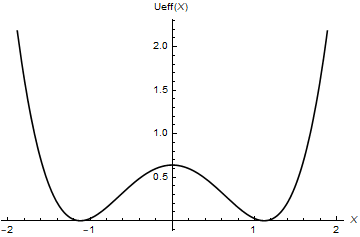
\includegraphics[scale=.7]{imagenes/sech-aprox.png}
    \caption{Forma de referencia del potencial efectivo para el caso de estudio $\epsilon=0.8$,$\gamma=0.64$ }.
    \label{fig:9.1}
\end{figure}

A partir de la forma del potencial efectivo se obtienen los puntos de equilibrio estable e inestables para el electrón, se encuentra que este efectuará oscilaciones alrededor de alguno de los puntos de equilibrio estable $X=\pm \sqrt{\epsilon/\gamma}$, con frecuencia de pequeñas oscilaciones:

\begin{equation}\label{eq:9.39}
    \omega_1=\frac{\sqrt{\gamma\epsilon}}{ m^*\omega}
\end{equation}

Se encuentran un punto de equilibrio inestable en $X=0$, y dos puntos de equilibrio estable en:

\begin{equation}\label{eq:9.40}
    X=\pm \sqrt{\frac{\epsilon}{\gamma}}
\end{equation}

Se ha hecho un diagrama de fases que permite observar de forma referencial, la evolución de la velocidad en función de la posición del electrón para distintas velocidades iniciales. Se puede observar que para velocidades iniciales pequeñas y en las cercanías de los puntos de equilibrio estable el electrón experimenta ciclos cerrados en el diagrama de fases, lo cual indica la presencia de oscilaciones alrededor de dichos puntos. Además se observa que para velocidades suficientemente grandes, el electrón realiza oscilaciones alrededor de $x=0$ pasando por los puntos de equilibrio estable e inestable en cada oscilación.

\begin{figure}[H]
    \centering
    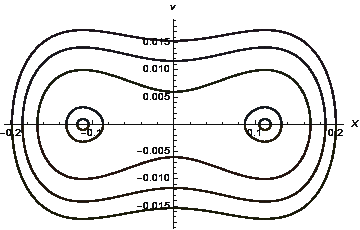
\includegraphics[scale=1]{imagenes/fase-clasico2.png}
    \caption{Diagrama de velocidad en función de la posición,$\epsilon=0.8$, $\gamma=0.64$, $\omega=100$ }
    \label{fig:9.2}
\end{figure}
